%%%%%%%%%%%%%%%%%%%%%%%%%%%%%%%%%%%%%%%%%%%%%%%%%%%%%%%%%%%%%%%%%%%%%%%%%%%%%%%%%%%%%%%%%%%
% Original author of template for CV (Plasmati Graduate CV v1.0 24/03/2013):
%  Alessandro Plasmati (alessandro.plasmati@gmail.com)
% Changes from the template onwards by (latest 30/01/2019):
% Pol del Aguila Pla (poldap@kth.se)
% Changes from the template onwards by (latest 14/02/2020):
% Joaquim Campos (joaquimcampos@duck.com)
% Downloaded from:
%  http://www.LaTeXTemplates.com
% License:
%  CC BY-NC-SA 3.0 (http://creativecommons.org/licenses/by-nc-sa/3.0/)
% Important note (PdaP):
%  This template needs to be compiled with XeLaTeX.
%  The main document font is called Fontin and can be installed in sudo-enabled
%  Linux systems by running fixFONTproblem.sh (will internally call sudo when necessary).
%%%%%%%%%%%%%%%%%%%%%%%%%%%%%%%%%%%%%%%%%%%%%%%%%%%%%%%%%%%%%%%%%%%%%%%%%%%%%%%%%%%%%%%%%%

%----------------------------------------------------------------------------------------
%	PACKAGES AND OTHER DOCUMENT CONFIGURATIONS
%----------------------------------------------------------------------------------------

% Font and paper size
\documentclass[a4paper,11pt]{article}

% Font loading
\usepackage{fontspec}
% \defaultfontfeatures{Mapping=tex-text}
% Set main font for document
% \setmainfont[SmallCapsFont = Fontin SmallCaps]{Fontin}
% Fonts are saved in /usr/share/fonts
% By order of preference
\setmainfont{Source Sans Pro}
% \setmainfont{Calibri}
% \setmainfont{Lato}
% \setmainfont{Roboto}
% \setmainfont{Fira Sans}
% \setmainfont{Montserrat}


\usepackage{bm}

% Formatting
\usepackage{xunicode,xltxtra,url,parskip}

% If then to toggle parts
\usepackage{ifthen}

% Coloring
\usepackage[usenames,dvipsnames]{xcolor}

% Margin specification
\usepackage{fullpage}

% Links and other clickable references
\usepackage{hyperref}
  % Link colors
  \definecolor{linkcolour}{rgb}{0,0.2,0.6}
  \hypersetup{colorlinks,breaklinks,urlcolor=linkcolour,linkcolor=linkcolour}

% Costumize section command
\usepackage{titlesec} % Used to customize the \section command
  % Text formatting
  \titleformat{\section}{\Large\raggedright}{}{0em}{}[\titlerule]
  % Spacing
  \titlespacing{\section}{0pt}{3pt}{3pt}

% Insert images
\usepackage{graphicx}

% Footnotes in tables
\usepackage{footnote}

% Tables that can span several pages
\usepackage{longtable}

% Several biblographies
\usepackage{bibunits}

% Trademark symbol
\usepackage{textcomp}

% enumerations
\usepackage{enumitem}

% Put references sections in the TOC (PDF and HTML links)
\usepackage[nottoc,numbib]{tocbibind}

\def\myname{Joaquim Campos}
\def\datespace{-2pt}
\def\title-main-sep{4pt}
\def\tabwidth{13cm}

\def\Techcv{true}
 % Includes \Techcv bool

\ifx\Techcv\empty
    % Code to execute if \Techcv is empty
    % \newcommand{\optExtraSpace}{}
    \newcommand{\sectionBioNonTech}{
      Outside the scope of my scientific expertise, I dedicate my time to exploring philosophy, psychology, meditation, ethics, and social systems. I find joy in tackling problems holistically, drawing inspiration from both ancient and modern wisdom, and considering the entire pipeline from philosophical and scientific inquiry to practical application. I appreciate engaging in thoughtful discussions, being exposed to different points of view, and—when suitable—sharing the little I know with others.

      Having started traveling at a young age, I've been fortunate to have explored more than 30 countries. I speak Portuguese and English fluently, have a conversational level of Spanish, and I can get by in French.
    }
    % \newcommand{\sectionTergar}{
    %   {\small Present} & Course in Philosophy and Meditation \\[\datespace]
    %   {\small \phantom{5}Sep 2023} & {\small \href{https://tergarinstitute.org/}{Tergar Institute}, Kathmandu, Nepal} \\[\title-main-sep]
    %   & {
    %   \parbox[t]{\tabwidth}{
    %   \footnotesize Head Teacher: Mingyur Rinpoche. \\
    %   Project: \href{https://joaquimcampos.com/madhyamaka}{Communicating Emptiness.} \\
    %   \emph{The course will continue on-site between mid-September and mid-December 2024.}
    %   }
    %   } \\
    %   \multicolumn{2}{c}{} \\
    % }
    % \newcommand{\mentionTergar}{at the Tergar Institute in Nepal }
    % \newcommand{\sectionDevOps}{}
    % \newcommand{\sectionVolunteering}{
    %   \vspace{15pt}

    %   \section{Volunteering}

    %   \vspace{4pt}
    %   \begin{itemize}
    %   \item In 2022, I spent one month teaching at \href{https://www.facebook.com/people/Charity-sammena-school-and-orphanage/100068066163936/}{Sammena school} in Arusha, Tanzania, to spend one month teaching at a local school. During my time there, I taught science, English, and mathematics to elementary and middle school students.
    %   % \vspace{5pt}\\
    %   \item Since 2021, I have been volunteering with \href{https://www.casa-apoioaosemabrigo.org/casa-a-associacao/}{CASA} whenever I am in Lisbon. The goal of this organization is to help alleviate the suffering of people experiencing homelessness. 
    %   \end{itemize}
    % }
\else
    % Code to execute if \Techcv is not empty
    % \newcommand{\optExtraSpace}{\vspace{5pt}}
    \newcommand{\sectionBioNonTech}{
      \vspace{10pt}
      %
      Highlights: \\[-20pt]
      \begin{itemize}[topsep=0pt, partopsep=0pt, parsep=0pt, itemsep=0pt, leftmargin=*]
        \item \href{https://www.joaquimcampos.com/pubs.html}{7 publications} with over 300 citations in top-tier venues, and 3 patents.
        \item Contributed to the development of \href{https://www.joaquimcampos.com/compression.html}{pioneering methods} in neural compression.
        \item Crafted \href{https://www.joaquimcampos.com/deepsplines.html}{novel algorithms} for
        % constructing sparse learning models and
        learning the activation functions of a neural network.
        \item Created the \href{https://pypi.org/project/deepsplines/}{"Deep Splines"} PyTorch package.
        \item Co-Founded \href{https://radiobooks.webflow.io/}{Radiobooks}—a startup that makes AI text-to-speech technology.
        \item Built the \href{https://github.com/joaquimcampos/radiobooks-sample}{back-end} of a complex text-to-speech app.
      \end{itemize}
    }
    % \newcommand{\sectionTergar}{}
    % \newcommand{\mentionTergar}{}
    % \newcommand{\sectionDevOps}{
    %   DevOps:       &  Python, C, FastAPI, Pytest, PyTorch, CI/CD, Bash, Linux, MongoDB, Docker, Github Actions, Codecov, AWS, Fly.io, Better Stack \vspace{5pt}\\
    % }
    % \newcommand{\sectionVolunteering}{}
\fi

\begin{document}

  % Remove page numbers
  \pagestyle{empty}

  %----------------------------------------------------------------------------------------
  %	NAME AND CONTACT INFORMATION
  %----------------------------------------------------------------------------------------

  % \begin{center}
  %   \begin{tabular}{lcr}
	%     \par{\Huge Joaquim Campos}\bigskip\par
  %     & & 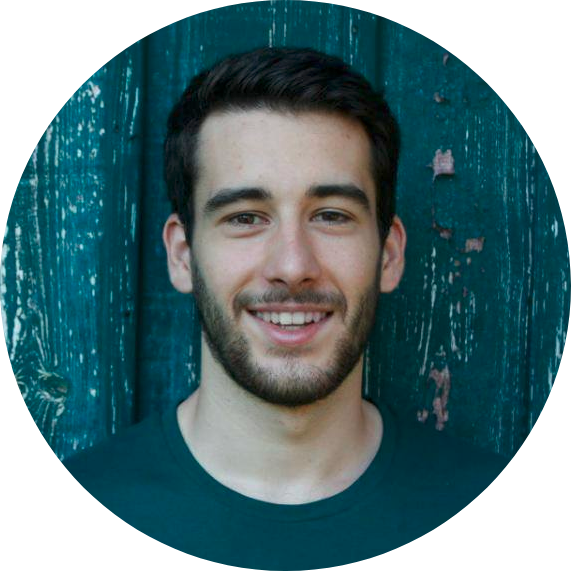
\includegraphics[width=0.2\textwidth]{../../images/Joaquim_circle.png}
  %     \\
  %   \end{tabular}
  % \end{center}
  \par{\Huge Joaquim Campos}\bigskip\par
  % Start picture environment at coordinates (0,0) relative to the bottom-left corner
  \begin{picture}(0,0)
    % Place image at coordinates (50, 100) from the bottom-left corner
    \put(300, -20){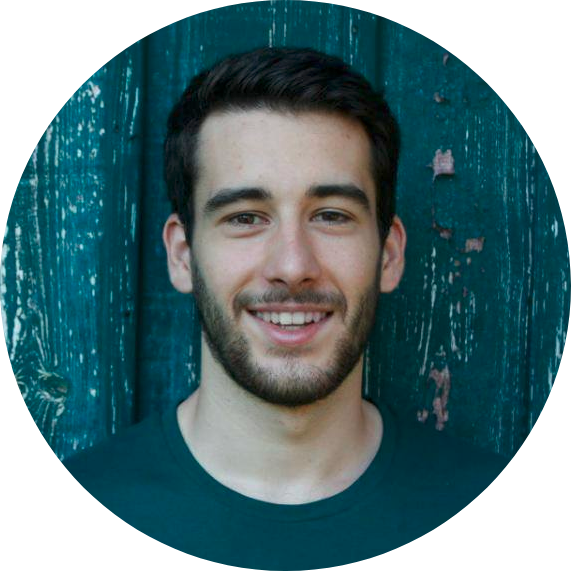
\includegraphics[width=4cm]{../../images/Joaquim_circle.png}}
  \end{picture}

  \vspace{15pt}

  \section{Personal data}

    \begin{tabular}{rl}
      Location: & Lisbon, Portugal \\
      % \textsc{Home address:} & Travessa da Cruz da Rocha 3, 4200-344, Porto, Portugal \\
      % \textsc{Mobile phone:} & +351 91-083-2298 \\
      Links: & \href{https://joaquimcampos.com}{Website} | \href{mailto:joaquimcampos@duck.com}{Email} | \href{https://scholar.google.com/citations?user=GT-VCroAAAAJ}{Google Scholar} |  \href{https://www.linkedin.com/in/joaquim-campos}{Linkedin} | \href{https://github.com/joaquimcampos/}{Github} \\
    \end{tabular}

  %----------------------------------------------------------------------------------------
  %  Summary
  %----------------------------------------------------------------------------------------

  \vspace{15pt}

  \section{In Brief}
    I am an engineer and researcher specializing in signal processing and artificial intelligence, as well as a Python developer. In academia, my focus has been on deep learning, learning theory, image and video compression, and inverse problems. Additionally, I am Co-Founder of Radiobooks, a startup that assists independent authors and self-learners in automatically converting their books into audiobooks using AI. Through this venture, I have gained knowledge in product development and Python DevOps.

    \sectionBioNonTech

    \vspace{4pt}

    \emph{Please note that I will be attending a course in philosophy and meditation at the Tergar Institute in Nepal between mid-September and mid-December in both 2024 and 2025.
    % As a result, I will not be able to work during those three months
    }

  %----------------------------------------------------------------------------------------
  %	EDUCATION
  %----------------------------------------------------------------------------------------
  \vspace{15pt}

  \section{Education}

    \begin{tabular}{r|p{\tabwidth}}

      {\small Present} & Course in Philosophy and Meditation \\[\datespace]
      {\small \phantom{5}Sep 2023} & {\small \href{https://tergarinstitute.org/}{Tergar Institute}, Kathmandu, Nepal} \\[\title-main-sep]
      & {
      \parbox[t]{\tabwidth}{
      \footnotesize Head Teacher: Mingyur Rinpoche. \\
      Project: \href{https://joaquimcampos.com/madhyamaka}{Communicating Emptiness.} \\
      \emph{The course will continue on-site between mid-September and mid-December 2024.}
      }
      } \\
      \multicolumn{2}{c}{} \\

      {\small Feb 2020} & MSc in Communication Systems \\[\datespace]
      {\small Sep 2016} & {\small \href{https://www.epfl.ch/en/}{EPFL} (École Polytechnique Fédérale de Lausanne), Lausanne, Switzerland
      } \\[\title-main-sep]
      & {
      \begin{minipage}[t]{\tabwidth}
        \footnotesize School: \href{https://www.epfl.ch/schools/ic/}{School of Computer and Communication Sciences}. \\
        Specialization: signal processing and artificial intelligence. \\
        % and their applications to imaging and audio
        Master's thesis: \href{https://www.joaquimcampos.com/assets/pubs/MSc_thesis.pdf}{Higher-Order Regularization Methods for Supervised Learning}. \\
        Grade: 5.67/6.00 — Ranking: 2nd/31.
      \end{minipage}
      } \\
      % Biomedical Imaging Group.
      % Supervisors and examiner: \textbf{Prof. Michael Unser, Shayan Aziznejad and Prof. François Fleuret}.
      %
      \multicolumn{2}{c}{} \\

      %------------------------------------------------
      {\small Jul 2016} & BSc in Electrical and Computer Engineering \\[\datespace]
      {\small Sep 2013} & {\small \href{https://www.ulisboa.pt/en}{Universidade de Lisboa}, Lisbon, Portugal} \\[\title-main-sep]
      & {
      \begin{minipage}[t]{\tabwidth}
        \footnotesize School: \href{https://tecnico.ulisboa.pt/en/}{Instituto Superior Técnico}. \\
        Grade: 16.4/20.00.
      \end{minipage}
      }
    \end{tabular}


  %----------------------------------------------------------------------------------------
  %  WORK EXPERIENCE
  %----------------------------------------------------------------------------------------

  \newpage

  \section{Work experience}

    \begin{tabular}{r|p{\tabwidth}}

      {\small Aug 2022} & Co-Founder and CTO \\[\datespace]
      % 2022 Aug 	& \emph{Converting books into audiobooks automatically using Artificial Intelligence}
      {\small Jan 2024} & {\small \href{https://radiobooks.webflow.io/}{Radiobooks}, Lisbon, Portugal} \\[\title-main-sep]
      & {
      \parbox[t]{\tabwidth}{
      \footnotesize Subject: Converting books into audiobooks automatically using Artificial Intelligence.
      \begin{itemize}[topsep=0pt, partopsep=0pt, parsep=0pt, itemsep=0pt, leftmargin=*, after=\vspace{0pt}]
        \item Designed and built an app for revising AI-generated audio.
        \item Tech stack: Python, FastAPI, MongoDB, Pytest, Docker, GitHub Actions, Codecov, Fly.io, AWS S3, and Better Stack.
      \end{itemize}
      }
      } \\
      \multicolumn{2}{c}{} \\

      %------------------------------------------------

      {\small Sep 2021} 	& Research and Teaching Assistant \\[\datespace]
      {\small Apr 2020} 	& {\small \href{https://bigwww.epfl.ch/}{Biomedical Imaging Group}, EPFL, Lausanne, Switzerland} \\[\title-main-sep]
      & {
        \parbox[t]{\tabwidth}{
        \footnotesize Subject: Supervised Learning with Sparsity-Promoting Regularization.
        \begin{itemize}[topsep=0pt, partopsep=0pt, parsep=0pt, itemsep=0pt, leftmargin=*, after=\vspace{0pt}]
          \item Developed a novel framework to learn the activation functions of a neural network;
          \item Designed a spline-based supervised learning method which constructs piecewise-linear models with few regions (sparse).
        \end{itemize}
        }
      } \\
      \multicolumn{2}{c}{} \\

      %------------------------------------------------
      {\small Aug 2018} & Research Intern \\[\datespace]
      {\small Mar 2019} &  {\small \href{https://studios.disneyresearch.com/}{Disney Research Studios}, Zurich, Switzerland}\\[\title-main-sep]
			& {
        \parbox[t]{\tabwidth}{
        \footnotesize Subject: Image and Video Compression using Deep Learning.
        \begin{itemize}[topsep=0pt, partopsep=0pt, parsep=0pt, itemsep=0pt, leftmargin=*, after=\vspace{0pt}]
          \item Developed the first content-adaptive neural image compression scheme;
          \item Aided in the construction of a state-of-the-art neural video compression framework.
        \end{itemize}
        }
      }
    \end{tabular}

  
  %
  %----------------------------------------------------------------------------------------
  %	TEACHING EXPERIENCE
  %----------------------------------------------------------------------------------------

  \vspace{15pt}

  \section{Teaching experience}

    \begin{tabular}{r|p{13cm}}

	  {\small Sep 2021} & Teaching Assistant in the Courses Signals and Systems I \& II \\[\datespace]
	  {\small Apr 2020} & \small{\href{https://www.epfl.ch/en/}{EPFL} (École Polytechnique Fédérale de Lausanne), Lausanne, Switzerland} \\[\title-main-sep]
    & {\footnotesize Taught by Prof. Michael Unser to the Life Sciences and Microenginneering sections.} \\
    % & \footnotesize{Approximate numbers per semester:
    %           $250$ students;
    %           $65\,\mathrm{h}$ of guidance of exercise sessions and interaction with students on the course forum;
    %           $60\,\mathrm{h}$ of class preparation; and
		% 					$40\,\mathrm{h}$ of exam supervision and grading.
    %           } \\

    \multicolumn{2}{c}{} \\

    {\small Sep 2021} & Supervision of Master Semester Projects \\[\datespace]
    {\small Apr 2020} & \small{\href{https://www.epfl.ch/en/}{EPFL} (École Polytechnique Fédérale de Lausanne), Lausanne, Switzerland} \\[\title-main-sep]
    & \footnotesize{Co-supervisor of two Master semester projects on \href{https://bigwww.epfl.ch/teaching/projects/abstract.html?f=00388}{lipschitz-constrained GANs}.} \\

    \end{tabular}

    %----------------------------------------------------------------------------------------
    % SKILLS
    %----------------------------------------------------------------------------------------

    \vspace{15pt}

    \section{Skills}

    \begin{tabular}{rp{13cm}}
  	Expertise:  & Theoretical and practical aspects of machine learning, deep learning, and signal processing; Python development.
    \vspace{5pt}\\
    DevOps:  &  Python, C, FastAPI, Pytest, PyTorch, CI/CD, Bash, Linux, MongoDB, Docker, Github Actions, Codecov, AWS, Fly.io, Better Stack \vspace{5pt}\\
    Languages: & Portuguese, English (professional), Spanish (advanced), French (conversational).
    % \vspace{5pt}\\
  	% Other skills: 	   & During my academic years, I developed valuable presentation, writing, and teaching skills, much of which I owe to Prof. Michael Unser.
    \end{tabular}

    \vspace{15pt}

      \section{Volunteering}

      \vspace{4pt}
      \begin{itemize}
      \item In 2022, I spent one month teaching at \href{https://www.facebook.com/people/Charity-sammena-school-and-orphanage/100068066163936/}{Sammena school} in Arusha, Tanzania, to spend one month teaching at a local school. During my time there, I taught science, English, and mathematics to elementary and middle school students.
      % \vspace{5pt}\\
      \item Since 2021, I have been volunteering with \href{https://www.casa-apoioaosemabrigo.org/casa-a-associacao/}{CASA} whenever I am in Lisbon. The goal of this organization is to help alleviate the suffering of people experiencing homelessness. 
      \end{itemize}

    %----------------------------------------------------------------------------------------
    %	LANGUAGES
    %----------------------------------------------------------------------------------------
      
    % \vspace{15pt}

    % \section{Languages}

    %   \begin{tabular}{rp{10cm}}

    %     Mother tongue: & Portuguese \\

    %     Professional (C1): & English \\

    %     Advanced (B2): & Spanish \\

    %     Conversational (B1): & French \\

    %   \end{tabular}

  %----------------------------------------------------------------------------------------
  %	PUBLICATIONS AND PATENTS
  %----------------------------------------------------------------------------------------

  \newpage

  \begingroup
  The publications can be consulted \href{https://joaquimcampos.com/pubs.html}{here}. \\[5pt]

  \begin{bibunit}[IEEEtran_Pol]
    \renewcommand\refname{Publications: Science}

    \nocite{
      goujonStableParameterizationContinuous2023,
      aziznejadMeasuringComplexityLearning2023,
      camposLearningContinuousPiecewiseLinear2022,
      bohraLearningActivationFunctions2020,
      aziznejadDeepNeuralNetworks2020,
      djelouahNeuralInterFrameCompression2019,
      camposContentAdaptiveOptimization2019}
    \putbib[../pubs/bibfile]

  \end{bibunit}

  \vspace{15pt}

  \begin{bibunit}[IEEEtran_Pol]
    \renewcommand\refname{Publications: Philosophy}

    \nocite{
      camposMahayanaBuddhistEthicsWork-in-Progress,
      camposWrongnessKillingNonHuman2018} %
    \putbib[../pubs/bibfile]

  \end{bibunit}

  \vspace{15pt}

  \begin{bibunit}[IEEEtran_Pol]
    \renewcommand\refname{Patents}

    \nocite{
      schroersContentAdaptiveOptimization2021,
      schroersSystemsMethodsReconstructing2021,
      schroersSystemsMethodsGenerating2021}
    \putbib[../pubs/bibfile]

  \end{bibunit}

  %----------------------------------------------------------------------------------------
  % INTERESTS AND ACTIVITIES
  %----------------------------------------------------------------------------------------

  % \vspace{-5pt}
  %
  % \section{Interests and activities}
  %
  % \section{On a Personal Note}
  %
  %   I meditate every morning. Cold showers clear my mind. Reader, especially about personal development, philosophy, psychology and society. When I have time a Pixar or Studio Ghibli movie, do Yoga or dancing. Productivity. I shut my cellphone during work and don't touch it on sundays. I practice a vegan lifestyle. I like to think deeply about topics and question my assumptions and beliefs. I work to be a positive influence am mindful of treating others with respect and compassion. I like to have my mind changed and engage in a healthy discussion. I have been fortunate enough to have traveled to abroad every year since I remember. I did competitive volleyball for $10$ years, swimming and represented Portugal at the I represented Portugal at the Youth World Padel Tournament in Mellilla in 2011. Music runs is a passion Piano or Guitar – 4 and 7 years of lessons, respectively.\\
  %
  % \section{Book list}
  %
  % \begin{tabular}{rp{10cm}}
  %
  %   \emph{The Righteous Mind} & by Jonathan Haidt \\
  %
  %   \emph{Animal Liberation} & by Peter Singer \\
  %
  % \end{tabular}
  %
  % \section{Traits}
  %
  % \begin{tabular}{rp{10cm}}
  %
  %   \emph{The Righteous Mind} & by Jonathan Haidt \\
  %
  %   \emph{Animal Liberation} & by Peter Singer \\
  %
  % \end{tabular}

\end{document}
